\begin{figure*}
%\begin{center}

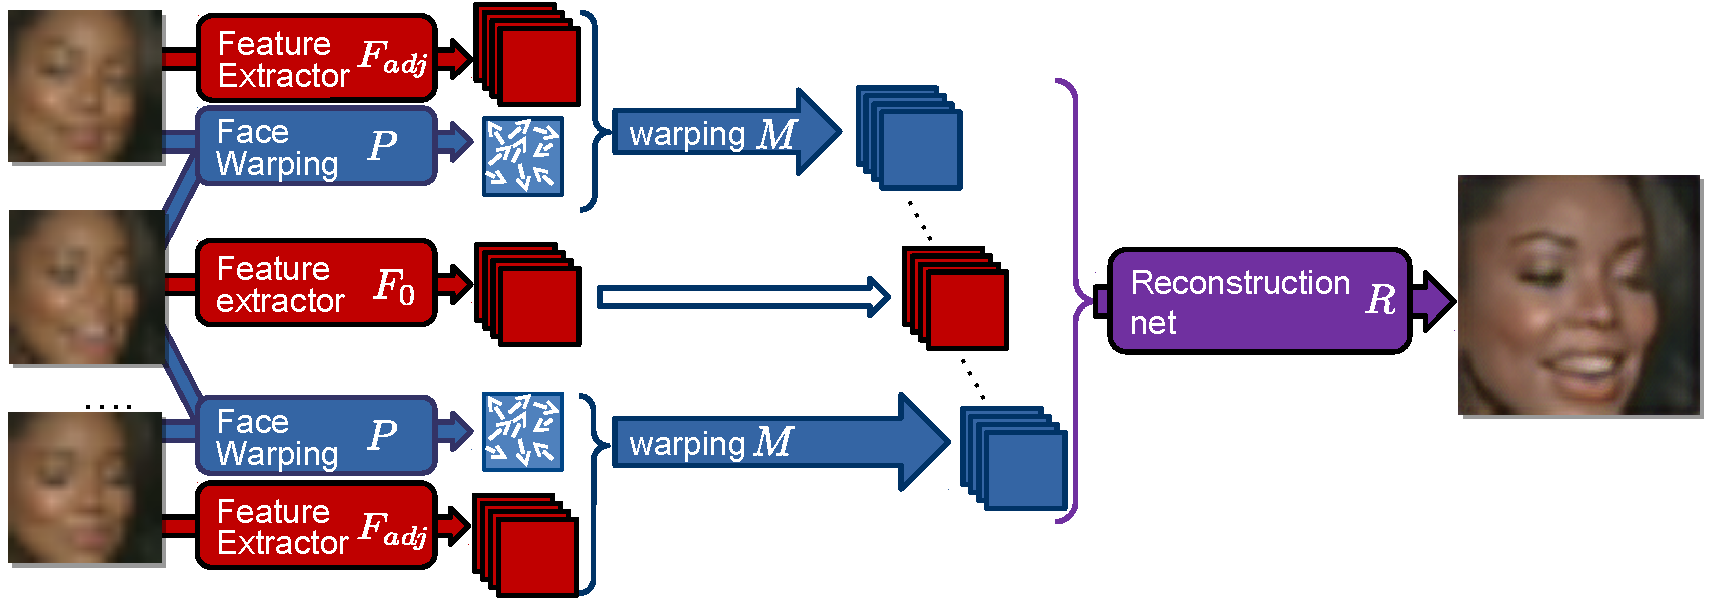
\includegraphics[width=\textwidth]{\srroot/images/method/superres_designations.pdf}

\caption{The general scheme of our video-based super-resolution convolutional network. \emph{Feature Extractor} modules (red) compute features for every frame in the input sequence, which are then warped by the \emph{Face Warping} sub-network (blue). The transformed feature maps are fed into the \emph{Reconstruction} sub-network (purple) that produces the central frame reconstruction. Spatial transformer modules \cite{JaderbergSZK15} with thin plate spline transformer are used in the \emph{Face Warping} sub-network.}

\label{fig:video}

%\end{center}

\end{figure*}

\subsection{Multi-frame face super-resolution}
%scheme
\label{sec:video}
Here we describe the proposed multi-frame face super-resolution convolutional neural network. Our architecture consists of three main learnable modules:
\begin{enumerate}
\item\emph{Feature Extractor} sub-network that computes features for every frame in the input sequence, \item\emph{Face Warping} sub-network that aligns input frames with the central frame,  
\item\emph{Reconstruction} sub-network that accepts warped features of input frames and perform reconstruction of the central frame in the sequence.
\end{enumerate}
The modules are combined as follows (\ref{fig:video}). \emph{Feature Extractor} outputs features for every frame in the input sequence. The feature maps are then warped by the \emph{Face Warping} sub-network. The transformed feature maps are fed into the \emph{Reconstruction} sub-network that produces the central frame reconstruction. Another option was to warp all the faces to match one standard pose, but as central frame warping may introduce additional distortions and loss of visual information, we only perform pairwise alignment between the central frame and other frames in the input sequence. 
%TODO can we actually perform warping??

In more detail, our goal is to restore the central frame $s_{0}$ of the input low-resolution sequence $s = [s_{-k}, ..., s_{0}, ..., s_{k}]$ of length $2k+1$. Here we work with RGB-images: $s_{i}\subseteq \mathbb{R}^{3\times h \times w}$, $i\subseteq [-k,..,k]$. We then start by processing each input frame $s_{i}$ with the feature extractor sub-networks $F_{i}$:
\begin{equation}
 f_{i} = F_{i}(\theta_{s_{i}}; F_{i}), 
 f_{i}\subseteq \mathbb{R}^{D\times {h}' \times {w}'}
\end{equation}
where $D$ is the number of output feature maps of size ${h}'\times{w}'$. Here all the feature extractors $F_{i}$ share parameters $\theta_{F_{i}}$, except for the feature extractor for the central frame $F_{0}$: $\theta_{F_{i}} == \theta_{F_{adj}}$, $F_{i} == F_{adj}$, where $i\subseteq [-k,..., -1, 1, ..., k]$. This is done for simplicity, and to avoid excessive memory consumption for long video-sequences.

To align all the adjacent frames $s_{i}$,  $i\subseteq [-k,..., -1, 1, ..., k]$, with the central frame $ s_{0}$, we incorporate the \emph{Face Warping} sub-network that consists of the learnable warping predictor $P(s_{0}, s_{i};\theta_{P})$ and the warping module $M(p_{i}, f_{i})$ that accepts transform parameters computed by $P$ and feature maps $F_{i}$. $M$ performs warping using differentiable sampling introduced in \cite{JaderbergSZK15}.

The warping predictor $P$ accepts frame pairs and outputs transform parameters $p_{i}$  that are used to warp each frame $s_{i}$, $i\neq0$, in the input sequence: 
\begin{equation}
    p_{i} = P(s_{0}, s_{i};\theta_{P}),
\end{equation}
where $i\subseteq [-k,..., -1, 1, ..., k]$.

Feature maps $f_{i}$ are transformed using warping parameters $p_{i}$ in differentiable manner \cite{JaderbergSZK15}: 
\begin{equation}
    f_{i}^{M}= M(p_{i}, f_{i}) = S(\mathcal{T}_{p_{i}}(G)), 
\end{equation}
where $i\subseteq[-k,..., -1, 1, ..., k]$, $\mathcal{T}$ is a predefined transform applied to the regular grid $G$ \cite{JaderbergSZK15}. Here we use Thin Plate Spline transform that is suitable for modeling non-rigid deformations inherent to face images. Therefore, $p_{i}\subseteq  \mathbb{R}^{2C\times 1 }$, where $C$ is a number of anchor points used for warping.

All the warped feature maps $f_{i}^M$ along with central frame feature map $f_{0}$ are then stacked together:
\begin{equation}
    f_{stacked}^{M} = [f_{-k}^{M}, ...,f_{0}, ..., f_{k}^{M}],
\end{equation}
 $f_{stacked}^{M} \subseteq  \mathbb{R}^{(2k+1)D\times {h}' \times {w}'}$.
 The resulting features $f_{stacked}^{M}$ are fed into \emph{Reconstruction} sub-network $R$, resulting in restored image $s_{N}^{R}$:
 \begin{equation}
 s_{0}^{R}=R(f_{stacked}^{M}; \theta_{R})
\end{equation}

The described architecture is learned in a supervised manner, using the loss function calculated for the ground truth image $s_{0}^{G}$ and the restored image $s_{0}^{R}$. The loss function is discussed in details in the section \ref{sec:loss}.



\subsection{Perceptual Loss for face super-resolution}

\label{sec:loss}
Perceptual losses have already been used for general super-resolution \cite{JohnsonAF16} and face frontalization \cite{cole2017face}. The idea is to compare high-level features for the ground truth image and the restored image in addition to pixel-level data. Here we use pre-trained VGG-face \cite{ParkhiVZ15} model (weights are fixed during training) to extract such features. The motivation behind such approach is that, first, less blurry results can be achieved \cite{JohnsonAF16}. Second, we use the pre-trained verification CNN for feature extraction, so there is a hope that our super-resolution neural network will be able to focus on facial features that are important for face identification. 
%The general scheme of the corresponding CNN 
%architecture (similar to \cite{JohnsonAF16}) is shown in Figure \ref{fig:vgg_loss}. 

%In general case there may be several perceptual loss terms that are added to form the final loss:
Our neural network described in the section \ref{sec:video} in learned using the following objective that includes pixel-level term along with sum of a number of feature-level terms:
\begin{equation}
\label{eq:loss}
\begin{aligned}
    L_{\theta_{F_{0}}, \theta_{F_{adj}}, \theta_{P}, \theta_{R}}(s_{-k}, ..., s_{0}, ..., s_{k}, s^{G}) = \\ \left \| s_{0}^{G} - s_{0}^{R}\right \|^{2}_{2} + \sum_{l \subseteq {layers}}  {\lambda_l \left \| s_{0,l}^{G} - s_{0,l}^{R}\right \|^{2}_{2}}
\end{aligned}
\end{equation}
where $s_{0}^{G}$ and $s_{0}^{R}$ are ground truth image and reconstruction for the frame $s_{0}$, $s_{0, l}^{G}$  and $s_{0, l}^{R}$ the features extracted by the layer $l$ of the ground truth image  $s_{0}^{G}$ and the restored image  $s_{0}^{R}$ accordingly, $\lambda_l$ is a fixed weight assigned to the corresponding loss components. Unlike \cite{cole2017face}, we use mid-level features extracted using VGG-face model as we observed that this leads to better results than using last fully connected layer of VGG-face.